\documentclass[assignment02_Solutions]{subfiles}

\IfSubStr{\jobname}{\detokenize{Solutions}}{\toggletrue{solutions}}{\togglefalse{solutions}}

\fancypagestyle{firstpage}

{\rhead{Assignment 2 \linebreak \textit{Version: \today}}}

\title{Assignment 2: Probabilistic Graphical Models}
\author{Machine Learning}
\date{Fall 2019}

\begin{document}

\maketitle
\thispagestyle{firstpage}


\begin{learningobjectives}
\bi
\item TODO
\ei
\end{learningobjectives}

\section{Motivation and Context}
\bi
\item We’ve learned how probabilities can be used to describe uncertainty in the world
\item We’ve learned how Bayes rule can be used to reason about hypotheses, models, or other things that cannot be directly observed.
\ei

\section{Generative versus Discriminative Models}
We should make more concrete the distinction between these two things.
p(y|x) versus p(x|y)p(y)

\section{Conditional Independence of Random Variables}

\section{Bayesian Networks}

\subsection{Simple Example}

\begin{center}
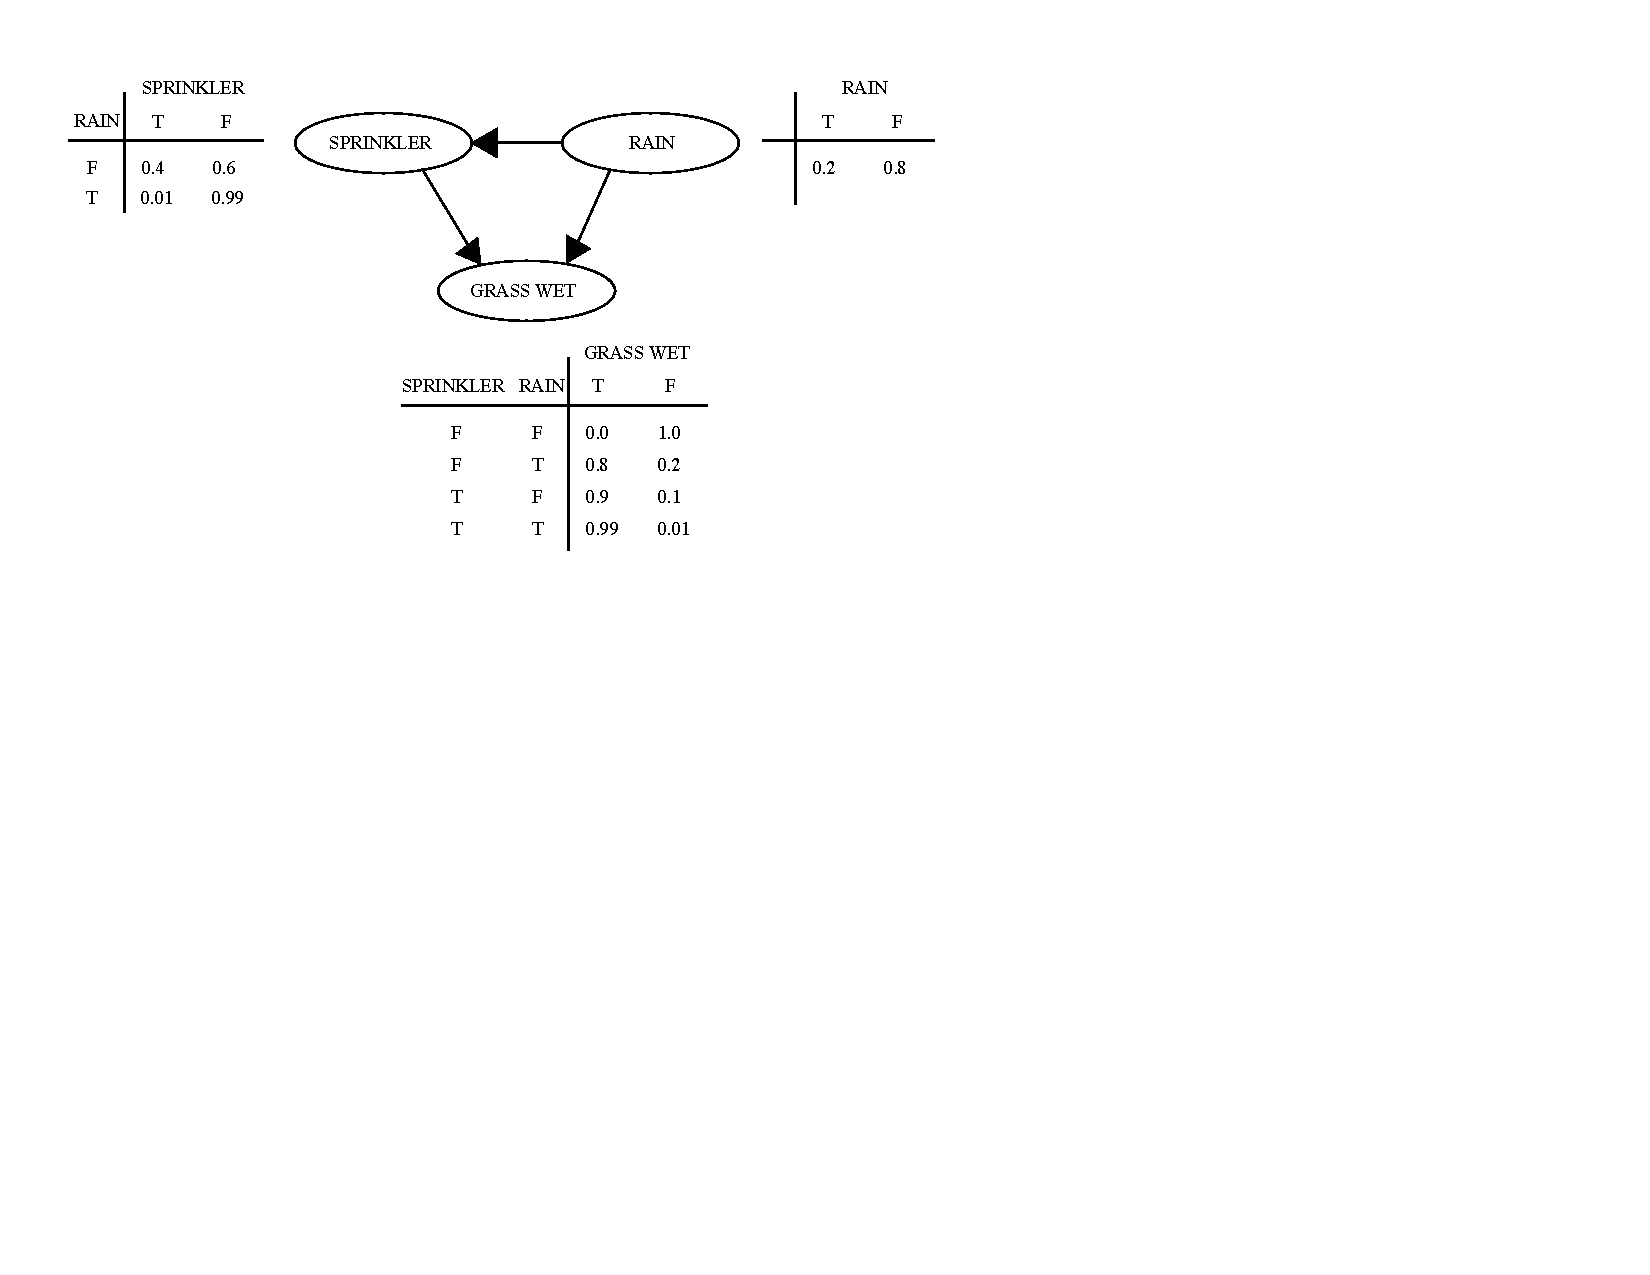
\includegraphics[width=0.7\linewidth]{figures/SimpleBayesNet}
\end{center}

\bi
\item Link to external resources
\item D-separation
\begin{externalresources}
Read \href{http://bayes.cs.ucla.edu/BOOK-09/ch11-1-2-final.pdf}{d-Separation without Tears}.
\end{externalresources}
\item State the main conditions
\item Do some exercises to determine when things are conditionally independent
\ei

\begin{exercise}
The alarm problem (need to find this one from CSE250A) (\href{http://aima.eecs.berkeley.edu/slides-pdf/chapter14a.pdf}{This has the description of the same network}).  \href{https://people.cs.pitt.edu/~milos/courses/cs2740/Lectures/class19.pdf}{More detail on the same network}.
\end{exercise}

\section{Na\"ive Bayes}
\begin{marginfigure}
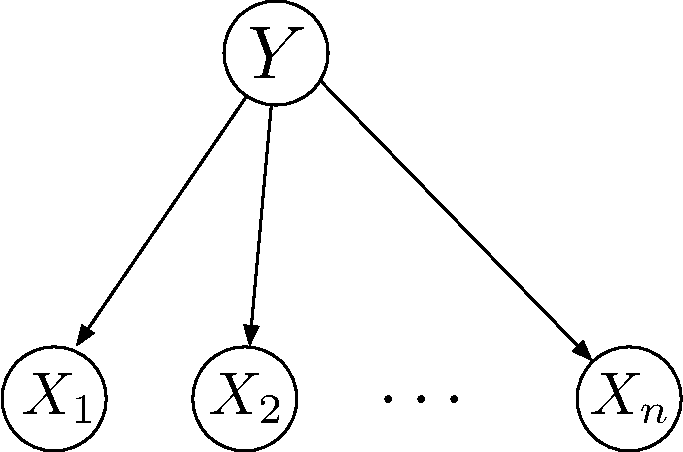
\includegraphics[width=\linewidth]{figures/naivebayesgm}
\end{marginfigure}

\section{Probabilistic frameworks for Fairness in ML}

\section{Compas Model of Recidivism}


\end{document}
